%~~~~~~~~ Chapter ~~~~~~~~
% ~~~~ Introduction ~~~~~~~~~~~~~~~~~~~~~~~~~~~~~~~~~~~~~~~~~~~~~~~~~~~~~~~~~~~~
\chapter{Introducción}
\label{ch:introduction_es}

% Kane Qspin
% hyperfine & exchange
% Qsimulator

El propósito inicial de esta tesis era la exploración de qubits de spines nucleares basados en grafeno. Esta idea se inspira en la propuesta para crear spines nucleares en Silicio, desarrollada por B. E. Kane\cite{Kane1988}, en 1988.

En el paper original el sistema propuesto consistía en donores de $\ce{P}$ en una matriz de $\ce{Si}$. Los donores de $\ce{P}$ tienen un spin nuclear $I=1/2$ y los estados electrónicos inducidos a su alrededor tienen un spin electrónico $S=1/2$.
El control entre ambos spines se proponía mediante un campo eléctrico en combinación con pulsos de micro- y radio-ondas.
El plan original era explorar la implementación de un sistema similar en un material completamente diferente: bicapas de grafeno hidrogenadas.
Sin embargo, mientras estudiabamos las interacciones de spin entre qubits, se nos ocurrió otra aplicación para este sistema: La simulación cuántica de modelos de red de fermiones que permiten el estudio de una clase muy amplia de propiedades electrónicas emergentes y además tiene perspectivas para aplicaciones a (más o menos) corto plazo.
\medskip

% The quantum information would be stored in the nuclear spin of $\ce{H}$ adatoms chemisorbed on top of bilayer graphene and in order to interact with it we propose the use of electric gating which it is known to control the band gap of the system and, with it, the hyperfine interaction as well as the exchange interaction among adatoms.
% \smallskip

Pero empecemos por el principio. Toda propuesta para crear qubits tiene que lidiar con dos requerimientos opuestos: la necesidad de que los qubits están totalmente aislados del entorno y la necesidad de que los qubits puedan interaccionar rápida y fuertemente cuando lo necesitemos, para poder leer y escribir información en ellos.
%~~~~~~~~~~~~~~~~~~~~~~~~~~ FIGURE ~~~~~~~~~~~~~~~~~~~~~~~~~%
\begin{wrapfigure}{R}{0.5\textwidth}
\centering
\vspace{-10pt}
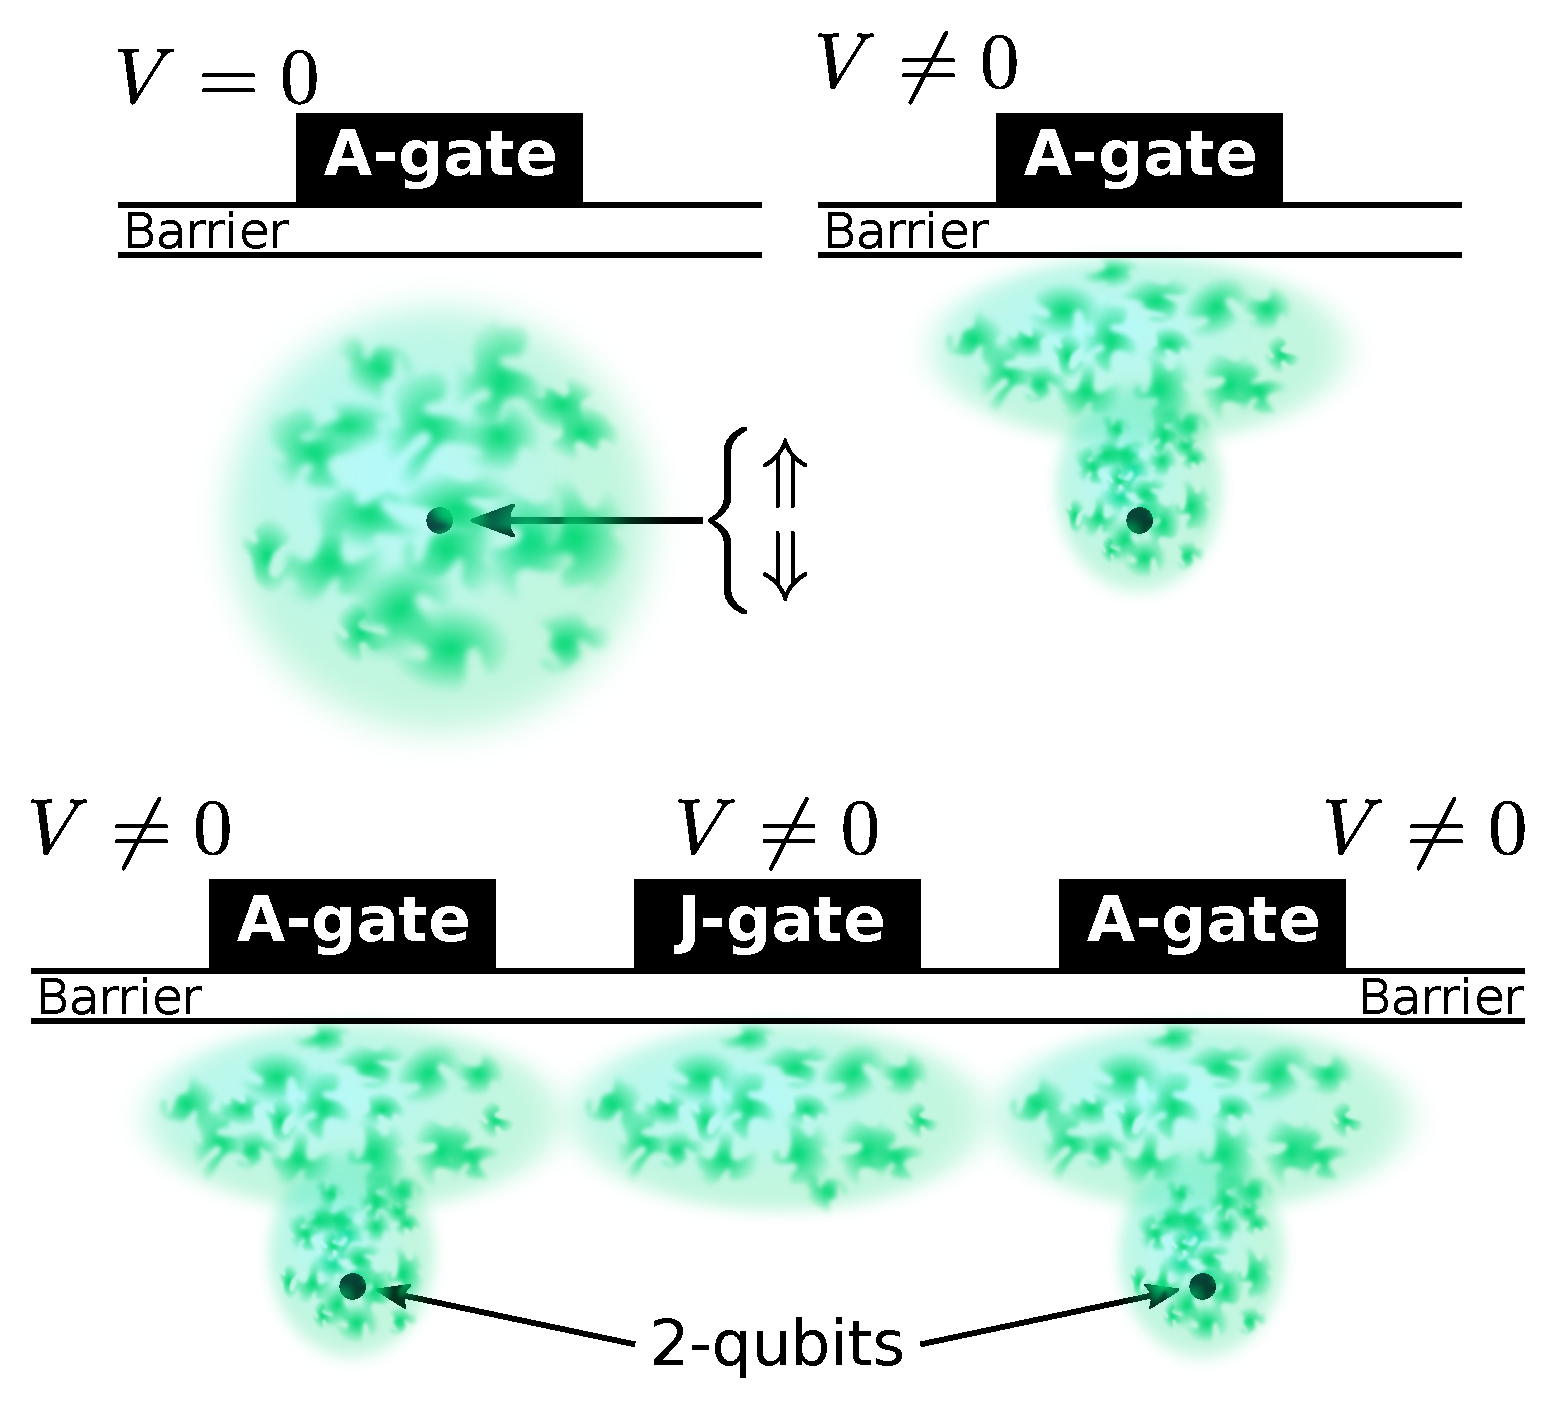
\includegraphics[width=0.45\textwidth]{introduction/figures/kane.pdf}
\vspace{-7pt}
\caption{Esquema de la propuesta de Kane para un ordenador cuántico de spines nucleares basado en silicio. Un campo eléctrico $A$ controla la interacción hiperfina al incrementar/reducir la densidad electrónica alrededor de los núcleos, permitiendo el aislamiento del spin nuclear cuando se requiera. Igualmente un campo eléctrico aplucado entre los qubits permitiría la interconexión de diferentes qubits}
\label{kane_proposal}
\end{wrapfigure}
\FloatBarrier
%~~~~~~~~~~~~~~~~~~~~~~~~~~~~~~~~~~~~~~~~~~~~~~~~~~~~~~~~~~~%
La propuesta de Kane\cite{Kane1988}, ``A Silicon-based nuclear spin quantum computer'' afronta el primer requerimiento de la siguiente forma: Lainformación cuántica se guarda en el spin nuclear de los átomos de fósforo insertados en una matriz de silicio ($\ce{Si}:\leftidx{^{31}}{\ce{P}}$). Se eligió el $\ce{Si}$ por su abundancia en forma de isótopos sin spin nuclear además de la enorme industria que tiene detrás, lo que asegura el conocimiento y las técnicas para manipular el material como se necesite. Una vez se eligió el material de la matriz no había muchas opciones para los donores. De hecho resulta que el único donor con spin nuclear $I=1/2$  es el fósforo\cite{Feher1959,Wilson1961} y, en particular, el isótopo $\leftidx{^{31}}{\ce{P}}$. Ademas varios estudios muestran que el tiempo de relajación de su spin nuclear puede exceder las 10 horas.\cite{Feher1959, Wilson1961, Waugh1988}

Cuando se introducen dopantes de $\ce{P}$ en $\ce{Si}$, se confina un electrón en su vecindad. La extensión del electrón localizado puede variar mucho, llegando a extendeers cientos de Ångströms por lo que, si hay varios dopantes en la misma zona, los estados electrónicos pueden actuar como un acoplo efectivo entre los spines nucleares\cite{Slichter1990}.

Esta aproximación al problema se aprovecha de lo débiles que son las interacciones con los spines nucleares por naturaleza así como de lo fácilmente manipulables que son los estados electrónicos confinados alrededor de los defectos.

Los procesos para controlar los qubits dependen de la implementacion. En la propuesta original se requería un contacto eléctrico sobre cada uno de los dopantes. La idea sería deformar la nube electrónica en la vecindad de los núcleos de $\ce{P}$ como se muestra en \fref{kane_proposal}. El principal efecto de esta deformación sería el incremento/reducción de la densidad electrónica alrededor del núcleo lo que incrementa/reduce la interacción hiperfina resultando en un desplazamiento de la frecuencia de resonancia para dar la vuelta al spin.

La interacción entre distintos qubits se podría apagar y encender usando los contactos eléctricos, aunque en realidad la implementación requiere que los dopantes estén a unas distancias muy específicas (con precisión atómica), lo que supone, sin duda, un problema en esta plataforma en particular. Igualmente la idea es incrementar/reducir la densidad electrónica en el espacio entre qubits para permitir/prevenir la propagación de la información de spin.

Otro gran reto es la detección del estado del spin de cada uno de los qubits en un momento dado. Aunque no hay una respuesta definitiva para este problema, hay muchas ideas para esquivarlo. La solución más simple es usar varios qubits en paralelo de forma que la magnetización macroscópica se pueda medir. Además, si los spines nucleares están incorporados en un aparato electrónico, es posible inferir el estado del spin nuclear basándose en propiedades electrónicas.\cite{Kane1992,Wald1994,Stich1996,Dixon1997,Dobers1988,Stegner2006}.

La implementación más puntera de este sistema ha demostrado ser capaz de leer (destructivamente) un único spin electrónico así como leer y manipular los spines de un sistema de dos qubits.\cite{Morello2010,Pla2012,Dehollain2014}


\section{Un qubit de spines nucleares basado en grafeno}
Nuestra propuesta reemplaza los \textbf{dopantes de $\ce{P}$} por \textbf{adátomos de $\ce{H}$ en bicapas de grafeno}.
El sistema tiene los mismos ingredientes: un material anfitrión, virtualmente, sin impurezas nucleares de spin,\footnote{La abundancia de isótopos de carbono con spin nuclear $I=0$ es $\sim98.9\%$ (que aún así podría ser problemático, aunque ese número para silicio es $\sim92.2\%$) pero, en principio, es factible conseguir sistemas de carbono isotópicamente puro.} un dopante con spin nuclear $I=1/2$ y un spin electrónico $S=1/2$ espacialmente confinado a su alrededor.


La interacción con las impurezas de spin nucleares en el material anfitrión son una fuente de decoherencia de spin bien conocida para los qubits de spin.\cite{khaetskii2002}
Por tanto la escasa existencia de isótopos de $\leftidx{^{13}}{\ce{C}}$ con spin nuclear $I=1/2$ hacen que grafeno sea una gran elección como material anfitrión para los qubits.

La interacción entre el spin nuclear y el electrónico, conocida como interacción hiperfina, es distinta de cero sólo para los orbitales $s$, y el nivel $1s$ es el que liga un electrón más cerca del núcleo, lo que hace del $\ce{H}$ un gran candidato.

A su vez, la quimisorción  de adtomos de $\ce{H}$ atrapa fuertemente el electrón con la nube $\pi$ de los electrones del grafeno, lo que saca la mayor parte del peso del orbital $s$. Por suerte la ocupación de dicho orbital es muy manipulable usando contactos eléctricos. Esta facilidad para manipularlo es un elemento clave para nuestra propuesta puesto que es el mecanismo que nos permitirá apagar y encender las interacciones de y entre qubits.
\smallskip


Los estados electrónicos en grafeno (y en la bicapa de grafeno) son muy manipulable. En concreto un campo eléctrico externo permite controlar propiedades muy relevantes para nuestra propuesta como la longitud de localización.


El motivo inicial para considerar la bicapa de grafeno fue la posibilidad de abrir un gap en las bandas al aplicar un campo eléctrico externo.\cite{McCann2006, Castro2007, Oostinga2007, Zhang2009, Taychatanapat2010, Castro2010a, Ponomarenko2011, Allen2012, Sui2015}.
Esta transición de conductor a aislante ofrece un mecanismo para controlar la longitud de localización de los estados electrónicos, lo que resulta en un control the la interacción efectiva electrón-electrónasí como de las interacciones con los spines nucleares.


Otra ventaja de usar adátomos de $\ce{H}$ sobre bicapas de grafeno en lugar de $\ce{Si}:\leftidx{^{31}}{\ce{P}}$ es que en la actualidad hay métodos para colocar los adátomos de $\ce{H}$ con precisión atómica y de manera reversible.\cite{elias2009,Brihuega2016,Brihuega2017} Específicamente unos 20 átomos de $\ce{H}$se han colocados en una única muestra de bicapa de grafeno y, en principio, no parece haber ninguna limitación física para colocar más átomos pues el proceso se podría automatizar para sistemas grandes.
\medskip
El estudio de cómo manipular las interacciones en este sistema nos llevó a darnos cuenta de que el sistema de adátomos de $\ce{H}$ sobre bicapas de grafeno ofrecen un campo de entrenamiento donde se pueden colocar estados electrónicos localizados donde se quiera y dondelas interacciones entre ellos se pueden manipular mucho con la aplicación de un campo eléctrico externo.
Un sistema como este es ideal para implementar realizaciones físicas de una gran variedad de Hamiltonianos: La meta última para simuladores cuánticos analógicos.
Nuestros análisis muestran que eligiendo con cuidado dónde depositar los adátomos (la distancia y posición relativa entre ellos) se pueden diseñar las interacciones elctrón-electrón para explorar tanto regímenes de interacción débil como fuerte.
\bigskip

Esta situación en la que podemos crear estados localizados donde queramos y controlar las interacciones electrón-electrón es especialmente atractiva tras el ``reciente'' descubrimiento de una fase de superconductividad no convencional en bicapas de grafeno rotadas\cite{Cao2018,Cao2018a}.
Aunque no discutiremos el tema en esta tesis, merece la pena señalar las similitudes entre nuestra propuesta y la física recién descubierta en las bicapas de grafeno rotadas.

Para conseguir superconductividad en bicapas de grafeno rotadas se requieren dos cosas. Primero, el ángulo de rotación tiene que ser muy pequño y tener un valor en concreto. Este requisito asegura la emergencia de un patrón de Moire que es responsable de la localización de los estados electrónicos en las fronteras entre dominios. Estos estados localizados resultan en la aparición de bandas casi planas por toda la zona de Brillouin y muy cercanas a la energía de Fermi. En segundo lugar el valor exacto del factor de llenado es clave para colocar el nivel de Fermi en medio de las bandas planas y así modificar la interacción electrón-electrón.
En el caso de bicapas rotadas, el diagrama de fases resultantes es bastante similar al de los cupratos lo que puede sugerir un mecanismo microscópico común para la superconductividad. La gran diferencia es que, mientras que los cupratos son materiales más o menos complejos, la químicadel grafeno se conoce muy bien desde hace mucho tiempo y el comportamiento de los orbitales $p$ del carbono (a diferencia de los orbitales $d$ en los cupratos) es mucho más simple.
El modelo efectivo a bajas energías del grafeno es probablemente el modelo más estudiado en las historia de la Física de la Materia Condensada, por lo que es esperable que el difícil problema de la superconductividad no convencional podría ser más fácil de estudiar en este caso.

Sin embargo, parece que la superconductividad no revelará sus secretos tan fácilmente puesto que, aunque el Hamiltoniano de bajas energías del grafeno está muy  bien entendido, su estensión a las bicapas rotadas no es tan fácil.

Probablemente es demasiado pronto para decir si la introducción de la superconductividad no convencional en la comunidad de grafeno/materiales bidimensionales puede ser un cambio radical para el problema centenario de la superconductividad.


\section{Ámbito de esta tesis}
La Física de la Materia Condensada es una rama inmensamente amplia de la Física. Engloba muchos sistemas diferentes a distintas escalas y con distintos métodos. Cubre desde las ideas más aplicadas de la metrología los conceptos matemáticos más profundos que subyacen el efecto Hall, clave para el Nobel de 2016.

Esta tesis pertenece a los métodos teóricos, y es principalmente computacional.
Estudiamos sistemas basados en grafeno desde un punto de vista teórico, usando métodos numéricos principalmente.
A lo largo de toda la tesis, la fuerza conductora ha sido tanto la posibilidad de resultados interesantes, independientemente de su ``inmediata'' aplicación, como la posibilidad de aplicaciones reales en el corto/medio plazo.
Esta posición, a medio camino entre investigación fundamenteal y aplicaciones en el mundo real ofrece una posición privilegiada para explorar temas interesantes sin perder contacto con la realidad experimental.
\bigskip

Esta tesis se centra en grafeno y sistemas relacionados, prestando especial atención a las aplicaciones de un caso particular: las bicapas de grafeno.

Es vox populi que la comunidad científica ha pasado una ``burbuja de interés'' respecto al grafeno y, como consecuencia, se ha promocionado como el material milagroso con potencial para cambiar el mundo tal y como lo conocemos. No voy a comentar la controversia de las todopoderosas propiedades del grafeno, pero sí que querría comentar brevemente la emoción por el grafeno dentro de la comunidad científica.
\smallskip

Para poder tener una descripción más o menos cuantitativa de la moda del grafeno he analizado el libro de abstracts del March Meeting de la APS desde 2005 hasta 2019 \footnote{Falta 2018 porque no conseguí encontrar el pdf del libro de abstracts completo. Aunque la edición de 2020 fue cancelada debido a la pandemia del covid19, el libro de abstracts estaba disponible, por lo que pudo ser incluido.}

El análisis contabiliza el número de abstracts que contienen una palabra (o grupo de palabras) y lo normaliza al número total de abstracts cada año.
Esta cantidad es una estimación de punto gordo, por supuesto, pero claramente este recuento está fuertemente relacionado con el interés de la comunidad de Materia Conodensada con cada tema.

%~~~~~~~~~~~~~~~~~~~~~~~~~~ FIGURE ~~~~~~~~~~~~~~~~~~~~~~~~~%
\begin{figure}[!ht]
\centering
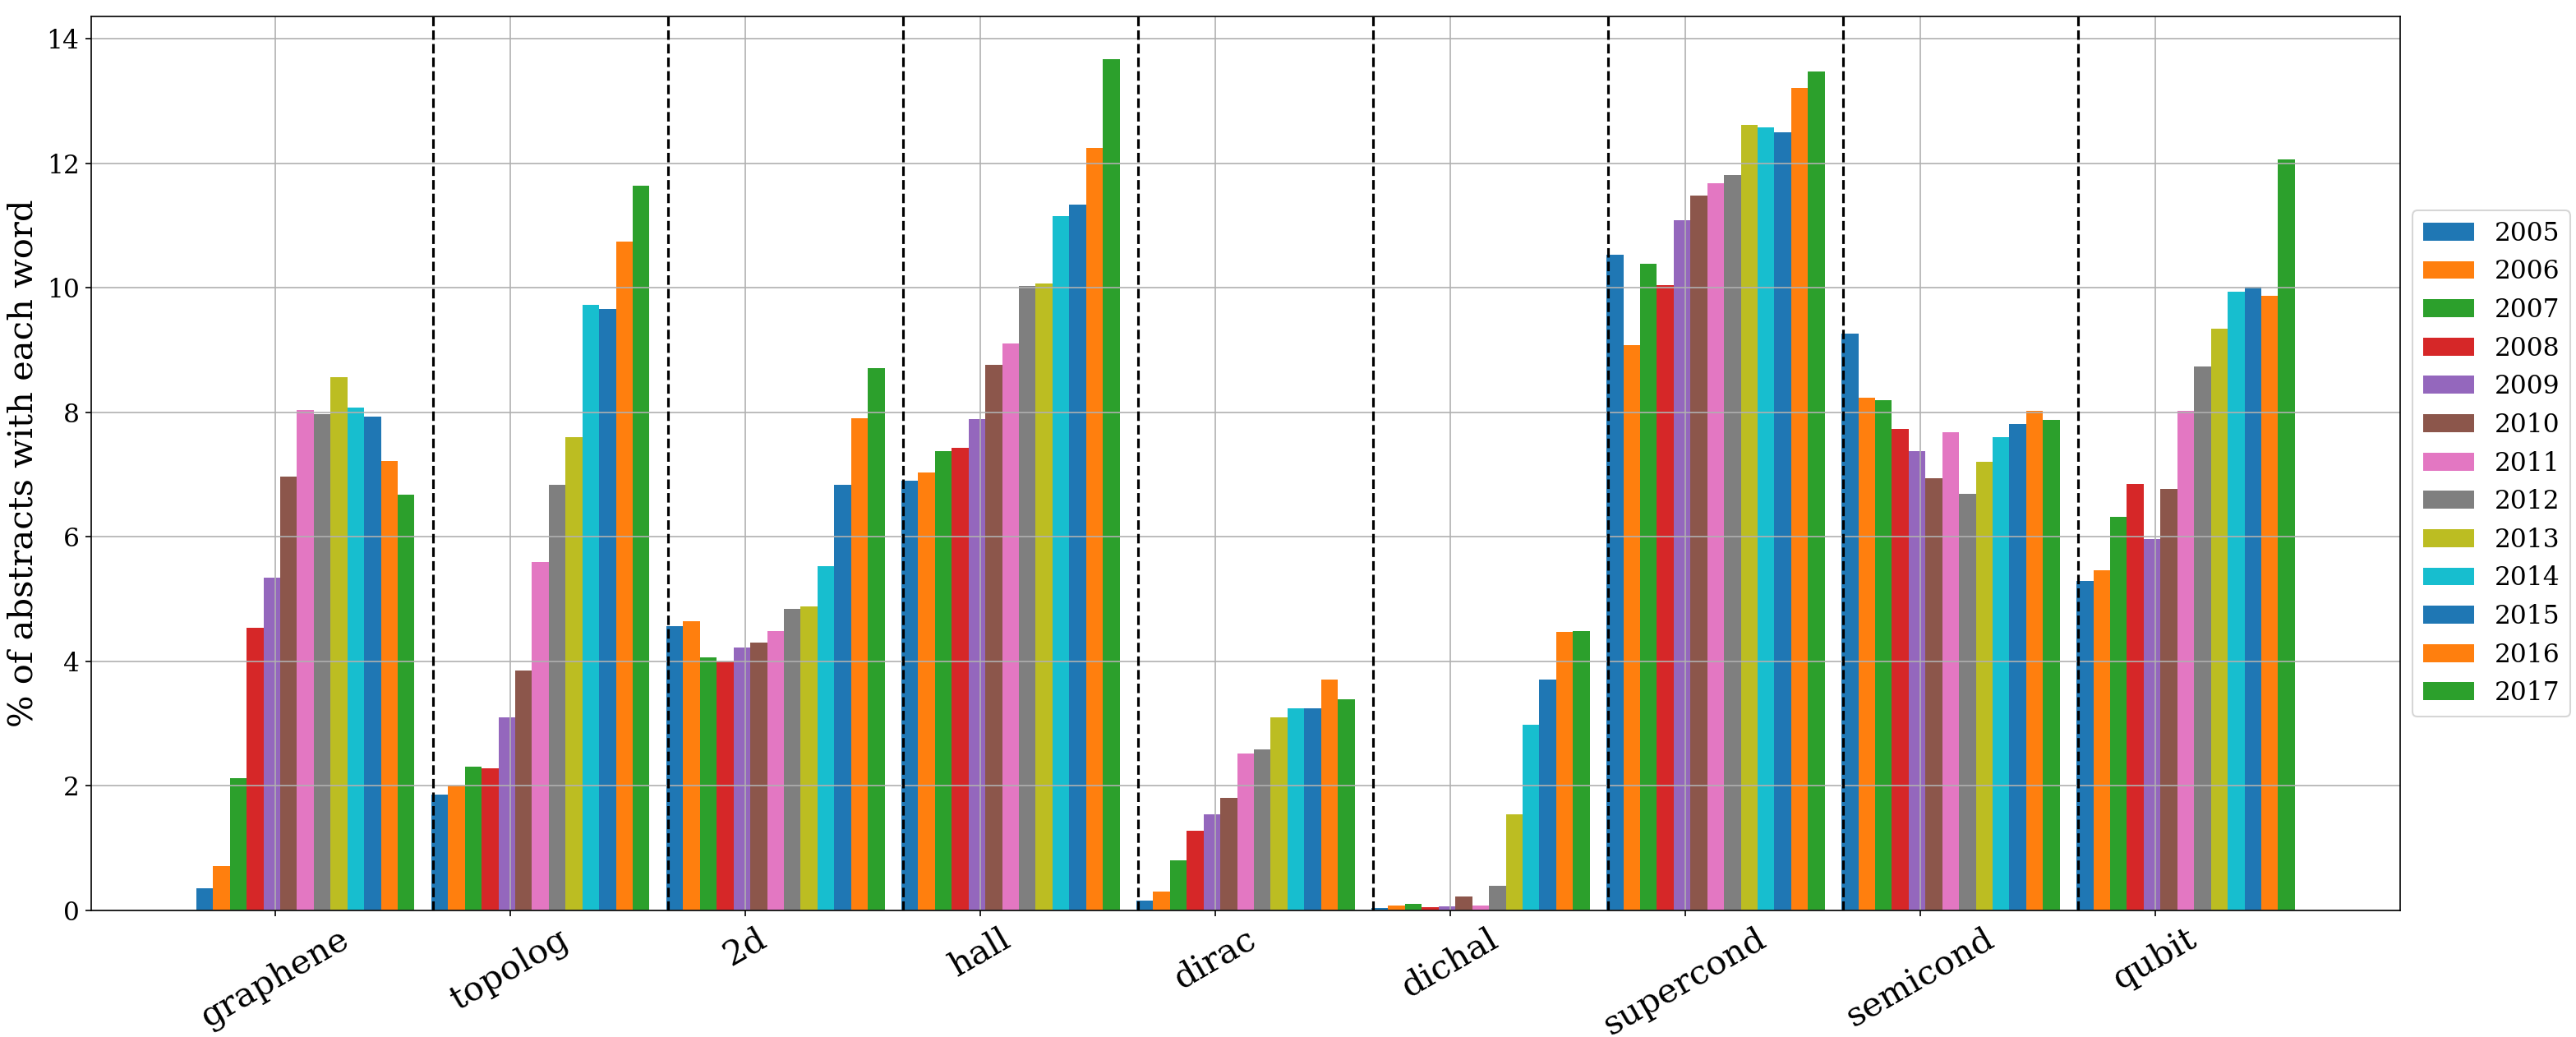
\includegraphics{introduction/figures/topics.png}
\vspace{-20pt}
\caption{Evolución a lo largo de los años de distintos temas en el March Meeting de la APS. El plot se ha hecho contando el número de abstracts que contienen una palabra y normalizando ese conteo por el número total de abstracts en cada conferencia. Hay que notar que las barras están colocadas en orden cronológico para cada término.}
\label{topics}
\end{figure}
%\FloatBarrier
%~~~~~~~~~~~~~~~~~~~~~~~~~~~~~~~~~~~~~~~~~~~~~~~~~~~~~~~~~~~%
En el caso de grafeno, el primer bloque de barras en \fref{topics}, se puede ver cómo crece en popularidad desde (casi) su descubrimiento y el comienzo de su decaimiento. Esta tendencia es un claro indicador de una posible ``burbuja de interés'', pero me gustaría señalar la evolución de los otros términos cercanos en in \fref{topics}: topolog\textcolor{gray}{[y,ical]}, 2d, dirac, \textcolor{gray}{quantum-,spin-,anomalous-}hall, dichal\textcolor{gray}{cogenides, $\ce{MoS2}$, $\ce{WS2}$, $\ce{WSe2}$}\footnote{Los términos en gris se agrupan durante el proceso de conteo de forma que se suman las apariciones de cada uno de ellos.}
Todos estos términos están indudablemente relacionados con grafeno y claramente muestran una tendencia creciente.
\medskip

Grafeno es muy interesante y probablemente se merezca toda la fama y atención que ha generado, pero yo diría que la verdadera importancia del grafeno reside en el hecho de que se ha convertido en el primer paso para el estudio de muchos otro materiales e incluso otras áreas de investigación.

La comprensión del grafeno ha sido la chispa que inició la investigación en materiales bidimensionales. \ac{2dm} son una familia de materiales muy interesantes tanto desde el punto de vista aplicado como desde la perspectiva de ciencia fundamental.

Por un lado, cualquier propiedad potencialmente útil, como la conductividad ajustable o el órden magnético, se convierte instantaneamente en interesante simplemente porque su naturaleza bidimensional asegura menores tamaños y quizás menores precios de posibles aparatos.
Por otro lado, su naturaleza bidimensional los coloca entre los regímenes clásico y cuántico: son macroscópicos (alguna vez extendiéndose hasta milímetros) pero al tener sólo un átomo de grosor hay efectos cuánticos por todas partes, lo que los hace fascinantes desde el punto de vista de la física fundamental.
Se han conseguido sintetizar muchos otros \ac{2dm} desde el grafeno: $\ce{MoS2}$, $\ce{WSe2}$, $\ce{MoTe2}$, $\ce{BN}$, $\ce{CrI3}$, $\ce{NbSe2}$, $\ce{TaS2}$, $\ce{MnBi2Te4}$... cada uno con su conjunto único de propiedades y su lista de posibles aplicaciones en el incipiente campo de las Tecnologías Cuánticas.
Algunos de estos materiales serán mencionados durante la tesis, pero el grafeno será el hilo conductor.
\bigskip

El resto de la tesis se estructura de la siguiente manera. \chref{ch:graphene} y \chref{ch:bilayer} repasan las propiedades básicas de la monocapa y la bicapa de grafeno respectivamente, así como la mayoría de los métodos de cálculo usados durante la tesis.

\chref{ch:vacancy} se basa en la publicación\onlinecite{Garcia-Martinez2017} y explora diversas propiedades de defectos $sp^3$ en grafeno.

\chref{ch:vacancy_bilayer} expande el estudio de los efectos de los defectos $sp^3$ a la bicapa de grafeno.

\chref{ch:hyperfine} explora la manipulabilidad del acoplo hiperfino del spin nuclear de los átomos de hidrógeno quimisorbidos en grafeno (y grafeno bicapa) como función del tamaño del gap de banda inducido eléctricamente.

\chref{ch:designer} estudia las posibilidades de los adátomos de $\ce{H}$ en la bicapa de grafeno como plataforma para realizar simulaciones cuánticas analógicas.
